\documentclass{article}
\usepackage{titlesec}

\usepackage[citestyle=authortitle-terse,backend=bibtex]{biblatex}
\addbibresource{bibliography.bib}

\setcounter{secnumdepth}{0}
\usepackage{sectsty}
\sectionfont{\fontsize{17}{20}\selectfont}

\usepackage[left=4cm, right=4cm]{geometry}
\usepackage{palatino,eulervm,dutchcal,xcolor}%fonts
\usepackage{graphicx,subcaption,float}
\usepackage{enumitem,parskip,multicol}
\usepackage{amsthm,amssymb,amsmath,mathtools,thmtools}
\usepackage{tikz,tikz-cd}
\usetikzlibrary{%
	matrix,%
	calc,%
	arrows,%
	shapes,
	decorations.markings,backgrounds,calc,intersections}
\tikzcdset{scale cd/.style={every label/.append style={scale=#1},
		cells={nodes={scale=#1}}}}
\usepackage[bookmarks,bookmarksopen,bookmarksdepth=3]{hyperref}
\hypersetup{%colores
	colorlinks=true,
	urlcolor=blue,
	linkcolor=magenta,
	citecolor=blue,
	filecolor=blue,
	urlbordercolor=white,
	linkbordercolor=white,
	citebordercolor=white,
	filebordercolor=white}
\usepackage{cleveref}
\Crefname{exercise}{Exercise}{Exercises}

\newcommand{\fakesection}[1]{%
	\par\refstepcounter{section}% Increase section counter
	\sectionmark{#1}% Add section mark (header)
	\addcontentsline{toc}{section}{\protect\numberline{\thesection}#1}% Add section to ToC
	% Add more content here, if needed.
}

\makeatletter %Hide section number
\def\@seccntformat#1{%
	\expandafter\ifx\csname c@#1\endcsname\c@section\else
	\csname the#1\endcsname\quad
	\fi}
\makeatother

\definecolor{blue-violet}{rgb}{0.54, 0.17, 0.89}
\definecolor{azure}{rgb}{0.0, 0.5, 1.0}
\definecolor{green(ncs)}{rgb}{0.0, 0.62, 0.42}
\definecolor{forestgreen}{rgb}{0.13, 0.55, 0.13}
\definecolor{limegreen}{rgb}{0.2, 0.8, 0.2}
\definecolor{palatinateblue}{rgb}{0.15, 0.23, 0.89}
\definecolor{trueblue}{rgb}{0.0, 0.45, 0.81}
\definecolor{goldenyellow}{rgb}{1.0, 0.87, 0.0}
\definecolor{fashionfuchsia}{rgb}{0.96, 0.0, 0.63}
\definecolor{brightcerulean}{rgb}{0.11, 0.67, 0.84}
\definecolor{jonquil}{rgb}{0.98, 0.85, 0.37}
\definecolor{lavendermagenta}{rgb}{0.93, 0.51, 0.93}
\definecolor{peru}{rgb}{0.8, 0.52, 0.25}
\definecolor{persimmon}{rgb}{0.93, 0.35, 0.0}
\definecolor{persianred}{rgb}{0.8, 0.2, 0.2}
\definecolor{persianblue}{rgb}{0.11, 0.22, 0.73}
\definecolor{persiangreen}{rgb}{0.0, 0.65, 0.58}
\definecolor{persianyellow}{rgb}{0.9, 0.89, 0.0}

\declaretheoremstyle[headfont=\color{trueblue}\normalfont\bfseries,]{colored1}
\declaretheoremstyle[headfont=\color{forestgreen}\normalfont\bfseries,]{colored2}
\declaretheoremstyle[headfont=\color{peru}\normalfont\bfseries,]{colored3}
\declaretheoremstyle[headfont=\color{persiangreen}\normalfont\bfseries,]{colored4}
\declaretheoremstyle[headfont=\color{brightcerulean}\normalfont\bfseries,]{colored5}
\declaretheoremstyle[headfont=\color{lavendermagenta}\normalfont\bfseries,]{colored6}
\declaretheoremstyle[headfont=\color{blue-violet}\normalfont\bfseries,]{colored7}
\declaretheoremstyle[headfont=\color{green(ncs)}\normalfont\bfseries,]{colored8}
\declaretheoremstyle[headfont=\color{peru}\normalfont\bfseries,]{colored9}
\declaretheoremstyle[headfont=\color{persiangreen}\normalfont\bfseries,]{colored10}

\declaretheorem[style=colored1,numberwithin=section,name=Theorem]{thm}
\declaretheorem[style=colored2,numberwithin=section,numberlike=thm,name=Proposition]{prop}
\declaretheorem[style=colored3,numberwithin=section,numberlike=thm,name=Lemma]{lemma}
\declaretheorem[style=colored4,numberwithin=section,numberlike=thm,name=Corollary]{coro}
\declaretheorem[style=colored5,numbered=no,name=Example]{example}
\declaretheorem[style=colored5,numbered=no,name=Examples]{exemplos}
\declaretheorem[style=colored7,numberwithin=section,name=Exercise]{exercise}
\declaretheorem[style=colored9,numbered=no,name=Remark]{remark}
\declaretheorem[style=colored9,numbered=no,name=Claim]{claim}
\declaretheorem[style=colored8,numbered=no,name=Definition]{defn}
\declaretheorem[style=colored10,numbered=no,name=Question]{question}

\newcommand{\R}{\mathbb{R}}
\newcommand{\Z}{\mathbb{Z}}
\newcommand{\N}{\mathbb{N}}
\newcommand{\C}{\mathbb{C}}
\newcommand{\Q}{\mathbb{Q}}
\newcommand{\D}{\mathbb{D}}
\newcommand{\T}{\mathbb{T}}
\renewcommand{\P}{\mathbb{P}}
\newcommand{\Ac}{\mathcal{A}}
\newcommand{\Bc}{\mathcal{B}}
\newcommand{\Cc}{\mathcal{C}}
\newcommand{\Dc}{\mathcal{D}}
\newcommand{\Ec}{\mathcal{E}}
\newcommand{\Fc}{\mathcal{F}}
\newcommand{\Gc}{\mathcal{G}}
\newcommand{\Lc}{\mathcal{L}}
\newcommand{\Oc}{\mathcal{O}}
\newcommand{\Qc}{\mathcal{Q}}
\newcommand{\Sc}{\mathcal{S}}
\newcommand{\Wc}{\mathcal{W}}
\newcommand{\mf}{\mathfrak{m}}
\newcommand{\gf}{\mathfrak{g}}
\newcommand{\X}{\mathfrak{X}}
\newcommand{\hf}{\mathfrak{h}}
\newcommand{\glf}{\mathfrak{gl}}
\newcommand{\of}{\mathfrak{o}}

\renewcommand{\Im}{\operatorname{Im}}
\renewcommand{\O}{\operatorname{O}}
\renewcommand{\S}{\mathbb{S}}
\renewcommand{\T}{\mathbb{T}}
\DeclareMathOperator{\Lie}{\operatorname{Lie}}

\DeclareMathOperator{\img}{img}
\DeclareMathOperator{\Arg}{Arg}
\DeclareMathOperator{\End}{End}
\DeclareMathOperator{\I}{I}
\DeclareMathOperator{\id}{id}
\DeclareMathOperator{\Id}{Id}
\DeclareMathOperator{\Alt}{Alt}
\DeclareMathOperator{\sgn}{sgn}
\DeclareMathOperator{\supp}{supp}
\DeclareMathOperator{\Int}{Int}
\DeclareMathOperator{\Ob}{Ob}
\DeclareMathOperator{\Mor}{Mor}
\DeclareMathOperator{\Top}{Top}
\DeclareMathOperator{\CGWH}{CGWH}
\DeclareMathOperator{\Hom}{Hom}
\DeclareMathOperator{\Map}{Map}
\DeclareMathOperator{\Tot}{Tot}
\DeclareMathOperator{\Vect}{Vect}
\DeclareMathOperator{\VectBund}{VectBund}
\DeclareMathOperator{\Open}{Open}
\DeclareMathOperator{\Ring}{Ring}
\DeclareMathOperator{\Set}{Set}
\DeclareMathOperator{\GL}{GL}
\DeclareMathOperator{\SL}{SL}
\DeclareMathOperator{\SO}{SO}
\DeclareMathOperator{\U}{U}
\DeclareMathOperator{\SU}{SU}
\DeclareMathOperator{\Sp}{Sp}
\DeclareMathOperator{\M}{M}
\DeclareMathOperator{\Aut}{Aut}
\DeclareMathOperator{\PGL}{PGL}
\DeclareMathOperator{\PSL}{PSL}
\DeclareMathOperator{\St}{St}
\DeclareMathOperator{\Vol}{Vol}
\DeclareMathOperator{\Length}{Length}

\begin{document}
\begin{minipage}{\textwidth}
	\begin{minipage}{.5\textwidth}
		Complex Manifolds in Dimension 1\\
	\end{minipage}%
	\begin{minipage}{.5\textwidth}
		\raggedleft
		Daniel González Casanova Azuela\par
		{\small\href{https://github.com/danimalabares/riemann-surfaces}{github.com/danimalabares/riemann-surfaces}}
	\end{minipage}%
\end{minipage}\vspace{.2cm}\hrule
\section{Home Assignment 5: Convergence for Lipschitz maps}
\setcounter{section}{5}
\begin{remark}
	For all metric spaces in this assignment, we assume that they admit a countable dense set (that is, are “second countable”).
\end{remark}
\begin{defn}
	A \textbf{\textit{path}} in a metric space $M$ is a continuous map $\gamma : [0, 1] \to M$. \textbf{\textit{Length}} of a path is $\sup_{0=x_1<\ldots<x_n=1\in[0,1]}\sum_{i=1}^nd(\gamma(x_i,x_{i+1}))$.
\end{defn}
\begin{exercise}
	Let $\gamma:[0,1]\to\R^2$ be a path of lenght 1, with $d(\gamma(0),\gamma(1))>1-\varepsilon^2$. Prove that the image of $\gamma$ is contained in a rectangle of size $\varepsilon\times(1+\varepsilon)$.
\end{exercise}
\textit{Attempt of solution.$\quad$}
	\iffalse Let $\gamma(x_0)$ be the point on $\img\gamma$ lying farthest from the segment joining $\gamma(0)$ and $\gamma(1)$, and call this distance $r$. Then $\img\gamma$ is contained in a square of $1\times 2r$ and  we have
	\begin{align*}
		1-\varepsilon^2<d(\gamma(0),\gamma(1))&\leq d(\gamma(0),\gamma(x_0))+d(\gamma(x_0),\gamma(1))<1
	\end{align*}\fi
	Consider the segment that joins $\gamma(0)$ and $\gamma(1)$ and the points of $\img\gamma$ that lie farthest from such segment to either side, call them $\gamma(x_1)$ and $\gamma(x_2)$. Call $r_1$ the distance between $\gamma(x_1)$ and the segment that joins $\gamma(0)$ to $\gamma(1)$, and $r_2$ accordingly. Then $\img\gamma$ is contained in a rectangle of size
	\begin{align*}
		d(\gamma(0),\gamma(1))&\times (r_1+r_2)\\
		>(1-\varepsilon^2)&\times (r_1+r_2)
	\end{align*}
	We want
	\begin{align*}
		(1-\varepsilon^2)(r_1+r_2)&<\varepsilon(1+\varepsilon)\\
		\iff r_1+r_2&<\frac{\varepsilon(1+\varepsilon)}{1-\varepsilon^2}
	\end{align*}
	The partition $0<x_1<x_2<1$ yields
	\begin{align*}
		1&\geq d(\gamma(0),\gamma(x_1))+d(\gamma(x_1),\gamma(x_2))+d(\gamma(x_2),\gamma(1))\\
		&\geq d(\gamma(0),\gamma(x_1))+r_1+r_2+d(\gamma(x_2),\gamma(1))
	\end{align*}
	so
	\begin{align*}
		1-d(\gamma(0),\gamma(x_1))-d(\gamma(x_2),\gamma(1))\geq r_1+r_2
	\end{align*}
	Projecting $\gamma(x_1)$ and $\gamma(x_2)$ onto the segment joining $\gamma(0)$ and $\gamma(1)$…
	\iffalse
	\begin{align*}
		1-\varepsilon^2<d(\gamma(0),\gamma(1))&=d(\gamma(0),\pi(x_0))+d(\pi(x_0),\pi(x_1))+d(\pi(x_1),\gamma(1))\\
		&=\sqrt{d(\gamma(0),\gamma(x_1))^2-r_1^2}\\
		&+d(\pi(x_0),\pi(x_1))\\
		&+\sqrt{d(\gamma(x_1),\gamma(1))^2-r_2^2}\\
	\end{align*}\fi
\begin{defn}
	A subset $X\subset \R^n$ has \textbf{\textit{measure zero}} if for every $\varepsilon > 0$, there exists a countable cover of $X$ by open rectangles $\{R_i\}$ such that $\sum\Vol(R_i)<\varepsilon$.
\end{defn}
\begin{exercise}
	Let $\gamma:[0,1]\to\R^2$ be a path of finite lenght. Prove that the image of $\gamma$ has measure 0.
\end{exercise}
\begin{proof}[Solution]
	{\color{red}How to apply the previous exercise? We may subdivide our path to pieces of length 1, but these do not necessarily satisfy that the distance betwen their endpoints is close to 1.}
	
	A simple argument found in \href{https://math.stackexchange.com/questions/2106497/fa-b-has-measure-zero/}{StackExchange} goes as follows. A path of finite length admits a reparametrization that is Lipschitz. Also, a Lipschitz function from $\R^2\to\R^2$ maps sets of measure zero to sets of measure zero. Then the function
	\begin{align*}
		[0,1]\times\{0\}&\to\R^2\\
		(t,0)&\mapsto\gamma(t)
	\end{align*}
	is Lipschitz, and since $[0,1]\times\{0\}$ has measure 0 in $\R^2$, so does $\img\gamma$.
	
	\iffalse
	 Suppose that $\gamma$ has length $L$ and let $\varepsilon>0$. Subdivide the image of $\gamma$ in $L/\varepsilon$ paths (or some close integer supposing $\varepsilon$ is small) in such way that we cover each of these smaller paths with a ball of diameter $L/\varepsilon$. The sum of the areas of these balls is a number close to $\frac{L}{\varepsilon}\cdot\pi\left(\frac{\varepsilon}{2}\right)^2=\frac{L\pi}{4}\varepsilon$. This number tends to zero as $\epsilon\to0$.\fi
\end{proof}
\begin{defn}
	Let $M$ be a metric space, and $\Map(X,M)$ the set of all continuous maps from a set $X$ to $M$. Define the metric on $\Map(X,M)$ using $d(f_1,f_2) = \sup_{x\in X} d(f_1(x), f_2(x))$. The corresponding topology is called the \textbf{\textit{uniform topology}} on $\Map(X,M)$.
\end{defn}
\begin{exercise}
	Prove that the length of a path is continuous in the uniform topology on $\Map([0,1],M)$, on the space $\Map_C([0,1],M)$ of $C$-Lipschitz paths, or find a counter-example.
\end{exercise}
\begin{proof}[Counter-example]
	Consider the path $\gamma_1(t)=(t,|t|)$ defined on $[-1,1]$. It is Lipschitz since
	\[d(\gamma_1(x),\gamma_1(y)=\|(x,|x|)-(y,|y|)\|\leq|x-y|+\Big||x|-|y|\Big|\leq|x-y|+|x-y|\leq2|x-y|.\]
	Now "fold" this path as in the figure. The new path $\gamma_2$ joins the points $(-1,1)$, $(-1/2,1/2)$, $(0,1)$, $(1/2,1/2)$ and $(1,1)$.
	\begin{figure}[H]
		\centering
		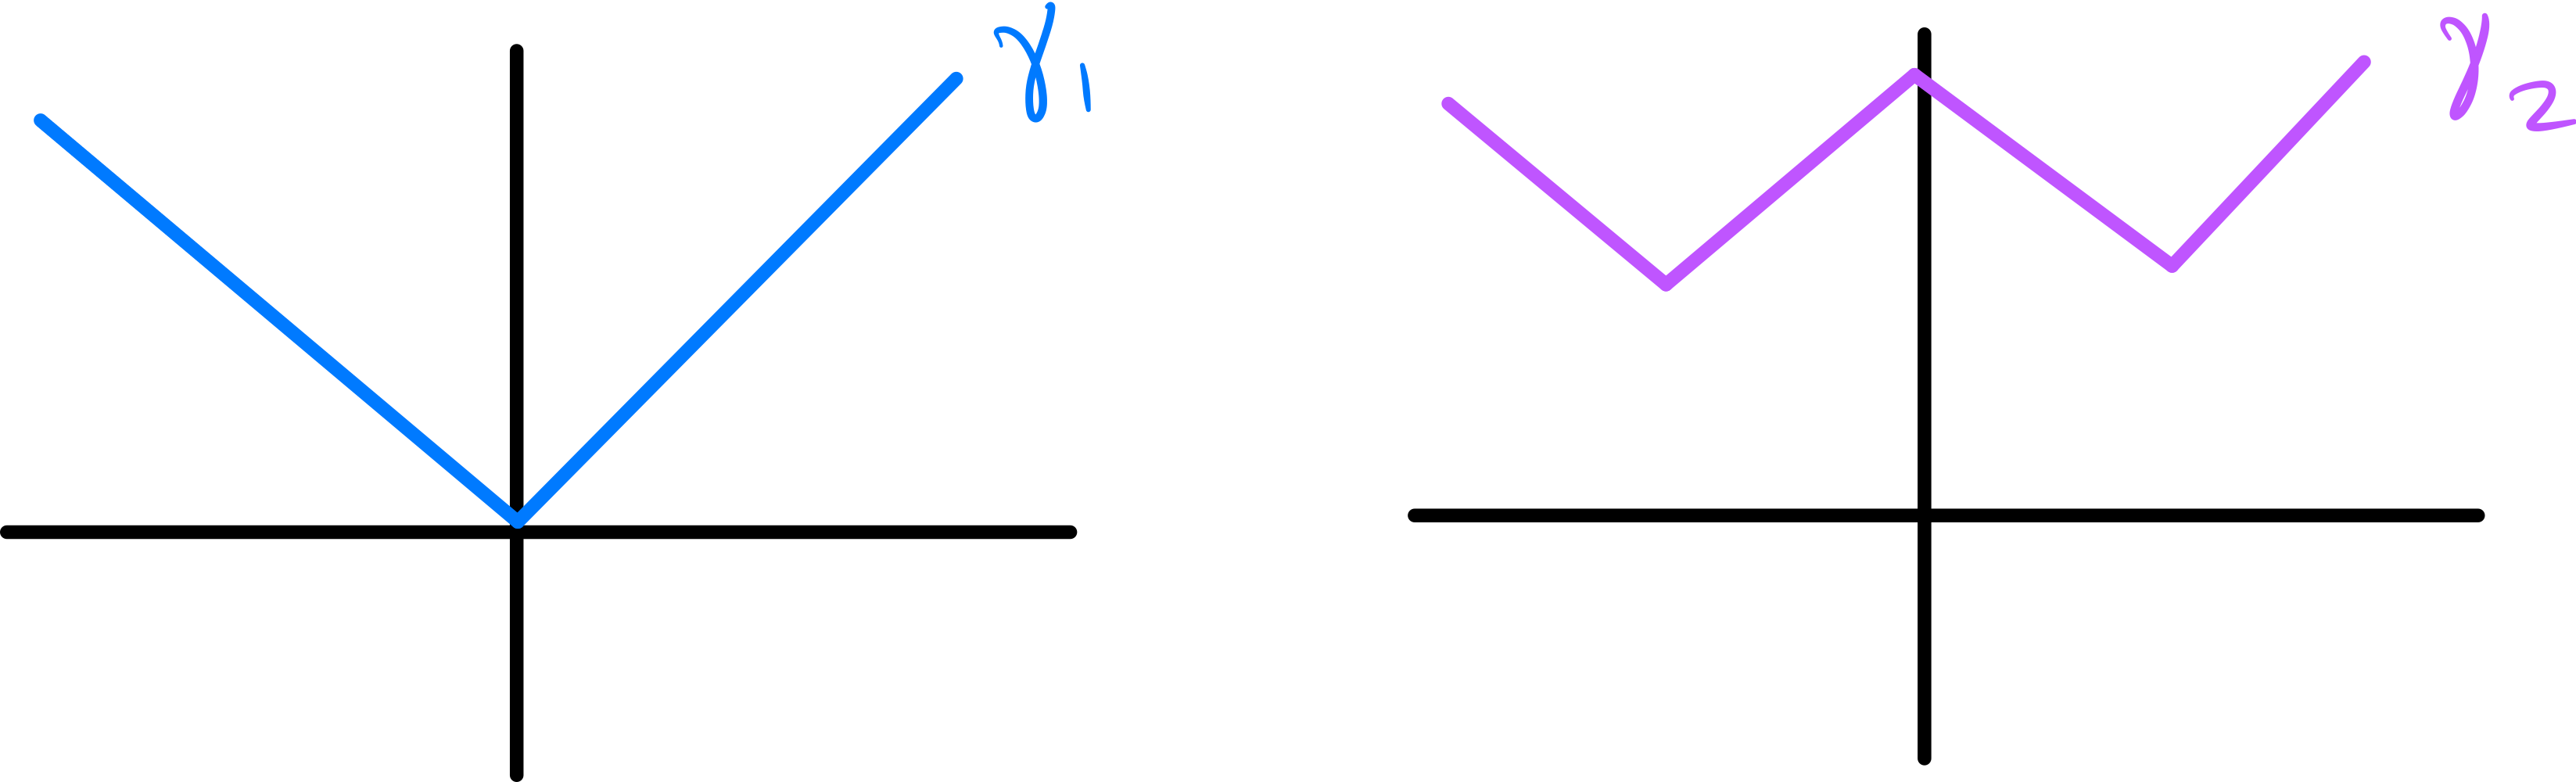
\includegraphics[width=0.7\linewidth]{lip}
	\end{figure}
	$\gamma_2$ has the same length as $\gamma_1$ and is also Lipschitz. Repeating this folding procedure produces a sequence of paths that tend to the horizontal segment joining $(-1,1)$ and $(1,1)$, but they have constant lenght greater than 2.	
\end{proof}

\begin{exercise}
	Let $M$ be a manifold with a marked point $m$, and $\Map((S^1, 0), (M, m))$ the space of maps putting $0 \in S^1$ to $m \in M$. We equip $\Map((S^1, 0), (M, m))$ with the uniform topology. Denote by $W$ the set of connected components of $\Map((S^1,0),(M,m))$. Construct a bijective equivalence between $W$ and the fundamental group $\pi_1(M, m)$.
\end{exercise}
\begin{proof}[Solution]
	Elements of $\Map((S^1,0),(M,m))$ are loops in $M$. A path in $\Map((S^1,0),(M,m))$ is an homotopy
	\[\Map((S^1,0),(M,m))\times [0,1]\to \Map((S^1,0),(M,m))\]
	Path-components in $\Map((S^1,0),(M,m))$ are homotopy classes of loops, that is, elements of $\pi_1(M,m)$. It suffices to show that path-components of $\Map((S^1,0),(M,m))$ coincide with its connected components with respect to the uniform topology.
	
	It is a standard fact that the compact-open topology on a space of maps is same as the uniform topology defined above when the source is compact and the target is metric, which is our case (prop. A.13 Hatcher).
	
	Further, $\Map((S^1,0),(M,m))$ with the compact-open open topology on is the well-known \textbf{\textit{loop space}} $\Omega(M)$, which is locally-path connected (at least when $M$ is a manifold, see \href{https://ncatlab.org/nlab/show/loop+space}{nLab "loop space"}), meaning path-connected components and connected componentes coincide.
\end{proof}

\begin{defn}
	Let $M$ be a topological space, and $U \subset M$ an open subset. Given $x \in X$, we define a subset $S_{x,U} \subset \Map(X,M)$ as the set of all maps putting $x$ to $U$. \textbf{\textit{Tychonoff topology}}, also called \textbf{\textit{topology of pointwise convergence}}, is topology where open subsets are obtained by finite intersections and all unions of $S_{x,U}$ for all possible $x$ and $U$.
\end{defn}

\begin{exercise}
	Let $\{f_i\} \in \Map(X,M)$ be a sequence of maps, with $M$ being a topological space. Prove that $\{f_i\}$ converges to $f$ in Tychonoff topology if and only if for each $x \in X$ one has $\lim_i f_i(x) = f(x)$.
\end{exercise}
\begin{proof}[Solution]
	Convergence in Tychonoff topology means that for every open set $V\subset\Map(X,M)$ containing $f$ there is a natural number $N$ such that for all $i>N$ every $f_i$ is in $V$. We may suppose that $V$ is of the form $S_{x,U}$ for some open set $U\subset M$ and $x\in M$.
	
	$(\impliedby)$ Suppose that for every $x\in X$ we have $\lim_if_i(x)=f(x)$. This means that for every open set $U\subset M$ containing $f(x)$ there is a natural number $N$ such that for all $i>N$ every $f_i(x)\in U$. This is just another way of saying that every $f_i$ is in $S_{x,U}$.
	
	 $(\implies)$ Now suppose $\{f_i\}$ converges to $f$ in Tychonoff topology. Let $x$ be any point of $X$ and let's prove that $\lim_if_i(x)=f(x)$. So let $U\subset X$ be an open set containing $f(x)$. Consider the set $S_{x,U}$, which is open in the Tychonoff topology of $\Map(X,M)$. Then there is $N$ such that for all $i>N$ every $f_i$ is in $S_{x,U}$. This just means that $f_i(x)\in U$ as required.
\end{proof}

\begin{exercise}
	Construct a sequence of functions $\{f_i \in C^\infty ([0, 1])\}$ which satisfy $\int_0^1|f_i(t)|dt = 1$ and converge pointwise to 0.
\end{exercise}
\begin{proof}[Solution]
	%\[\int_0^1x^{n}dx=\left[\frac{x^{n+1}}{n+1}\right]_0^1=\frac{1}{n+1}\]
	For every $n\in\N$ and real number $\alpha_n$ there exists a $C^\infty$ bump function that is $\alpha_n$ in a neighbourhood of $1/n$ and has support in $\left(\frac{1}{n}-\frac{1}{2n},\frac{1}{n}+\frac{1}{2n}\right)$. By intermediate value theorem we can choose $\alpha_n$ such that its integral is exactly 1. The sequence of these functions satisfies the required contitions.
\end{proof}

%\printbibliography
\end{document}